%!TEX program = xelatex
\documentclass[9pt, compress]{beamer}
\usetheme[titleprogressbar]{m}

\usepackage{array}
\usepackage{tabu}
\usepackage[english,russian]{babel} 
\usepackage{longtable} %tabu needs this to be loaded.
\usepackage{lipsum}

\usepackage{rotating}
\usepackage{graphicx}
\usepackage{color}
\usepackage{xcolor}
\usepackage{xcolor,colortbl}
\usepackage{listings}
\usepackage{sectsty}
\usepackage{caption}


\DeclareCaptionFont{white}{\color{white}}
\DeclareCaptionFormat{listing}{\colorbox{gray}{\parbox{\dimexpr\textwidth-1.72\fboxsep\relax}{#1#2#3}}}
\captionsetup[lstlisting]{format=listing,labelfont=white,textfont=white,margin=0pt}
\lstset{language=C,
	basicstyle=\footnotesize,
	keepspaces=true,
	numbers=left,
	tabsize=4,               
	frame=single,                           % Single frame around code
	rulecolor=\color{black},
	captionpos=b,
	showstringspaces=false,	
	abovecaptionskip=-0.9pt,
	xleftmargin=3.4pt,
	xrightmargin=2.6pt,
	breaklines=true,
	postbreak=\raisebox{0ex}[0ex][0ex]{\ensuremath{\color{black}\hookrightarrow\space}},
	xleftmargin=3.2pt,
	literate={а}{{\selectfont\char224}}1
	{~}{{\textasciitilde}}1
	{б}{{\selectfont\char225}}1
	{в}{{\selectfont\char226}}1
	{г}{{\selectfont\char227}}1
	{д}{{\selectfont\char228}}1
	{е}{{\selectfont\char229}}1
	{ё}{{\"e}}1
	{ж}{{\selectfont\char230}}1
	{з}{{\selectfont\char231}}1
	{и}{{\selectfont\char232}}1
	{й}{{\selectfont\char233}}1
	{к}{{\selectfont\char234}}1
	{л}{{\selectfont\char235}}1
	{м}{{\selectfont\char236}}1
	{н}{{\selectfont\char237}}1
	{о}{{\selectfont\char238}}1
	{п}{{\selectfont\char239}}1
	{р}{{\selectfont\char240}}1
	{с}{{\selectfont\char241}}1
	{т}{{\selectfont\char242}}1
	{у}{{\selectfont\char243}}1
	{ф}{{\selectfont\char244}}1
	{х}{{\selectfont\char245}}1
	{ц}{{\selectfont\char246}}1
	{ч}{{\selectfont\char247}}1
	{ш}{{\selectfont\char248}}1
	{щ}{{\selectfont\char249}}1
	{ъ}{{\selectfont\char250}}1
	{ы}{{\selectfont\char251}}1
	{ь}{{\selectfont\char252}}1
	{э}{{\selectfont\char253}}1
	{ю}{{\selectfont\char254}}1
	{я}{{\selectfont\char255}}1
	{А}{{\selectfont\char192}}1
	{Б}{{\selectfont\char193}}1
	{В}{{\selectfont\char194}}1
	{Г}{{\selectfont\char195}}1
	{Д}{{\selectfont\char196}}1
	{Е}{{\selectfont\char197}}1
	{Ё}{{\"E}}1
	{Ж}{{\selectfont\char198}}1
	{З}{{\selectfont\char199}}1
	{И}{{\selectfont\char200}}1
	{Й}{{\selectfont\char201}}1
	{К}{{\selectfont\char202}}1
	{Л}{{\selectfont\char203}}1
	{М}{{\selectfont\char204}}1
	{Н}{{\selectfont\char205}}1
	{О}{{\selectfont\char206}}1
	{П}{{\selectfont\char207}}1
	{Р}{{\selectfont\char208}}1
	{С}{{\selectfont\char209}}1
	{Т}{{\selectfont\char210}}1
	{У}{{\selectfont\char211}}1
	{Ф}{{\selectfont\char212}}1
	{Х}{{\selectfont\char213}}1
	{Ц}{{\selectfont\char214}}1
	{Ч}{{\selectfont\char215}}1
	{Ш}{{\selectfont\char216}}1
	{Щ}{{\selectfont\char217}}1
	{Ъ}{{\selectfont\char218}}1
	{Ы}{{\selectfont\char219}}1
	{Ь}{{\selectfont\char220}}1
	{Э}{{\selectfont\char221}}1
	{Ю}{{\selectfont\char222}}1
	{Я}{{\selectfont\char223}}1,
	extendedchars=true
}
\usepackage{textpos}
\newcommand<>{\fullsizegraphic}[1]{
  \begin{textblock*}{0cm}(-1cm,-3.78cm)
  \includegraphics[width=\paperwidth]{#1}
  \end{textblock*}
}

%галочка
\usepackage{amssymb}% http://ctan.org/pkg/amssymb
\usepackage{pifont}% http://ctan.org/pkg/pifont
\newcommand{\cmark}{\ding{52}}%
\newcommand{\xmark}{\ding{56}}


\usepackage{booktabs}  
\usepackage[scale=2]{ccicons}
\usepackage{minted}
\usepgfplotslibrary{dateplot}
\usemintedstyle{trac}
\author{Студент: \textbf{Д.В. Круминьш}\\ 
	Группа: \textbf{13541/3}\\ \\
	Преподаватель: \textbf{Е.В. Душутина} }
\title{Системная изоляция процессов в Windows средствами LPAC}
\subtitle{Курс: \textbf{Проектирование ОС и компонентов}}
%\logo{123}
\institute{Санкт-Петербургский политехнический университет Петра Великого}
\date{ }
%\subject{}
%\setbeamercovered{transparent}
%\setbeamertemplate{navigation symbols}{}
\begin{document}
	\maketitle
%	\begin{frame}
%		\frametitle{Оглавление}
%		\tableofcontents{}
	%\end{frame}
	
\section{ТЕОРИЯ}


\begin{frame}[fragile]
\frametitle{Причины потребности в изоляции}
Современные серверы обладают избыточной производительностью, и приложения порой не используют даже их части.

Выходом стала \textbf{виртуализация}, позволяющая запускать несколько ОС на одном сервере, гарантированно разделяя их между собой и выделяя каждой нужное количество ресурсов.

Следующий этап — \textbf{микросервисы}, когда каждая часть приложения развертывается отдельно, как самодостаточный, изолированный компонент.

В ОС семейства \textbf{Windows} данным инструментом служит - \textbf{Application Container}.
\end{frame}


\begin{frame}[fragile]
\frametitle{Application Container}
\textbf{Application Container} - это иной тип виртуализации, предоставляющий обособленную среду для выполнения приложений, называемую OS Virtualization. Реализуются контейнеры за счет использования изолированного пространства имен, включающего все необходимые для работы ресурсы (виртуализированные имена), с которыми можно взаимодействовать (файлы, сетевые порты, процессы и прочее) и выйти за которые нельзя.

Контейнеры используют одно и то же \textbf{ядро ОС}. В отличие от виртуальных машин, контейнеры не полагаются на отдельный \textbf{слой гипервизора}.

Приложение внутри контейнера считает, что оно единственное, и работает в полноценной ОС без каких-либо ограничений. 
\end{frame}

\begin{frame}[fragile]
\frametitle{Упрощенный пример контейнеризации}
\begin{figure}
\centering
\begin{minipage}{.2\textwidth}
  \centering
  
\includegraphics[width=.9\linewidth]{img/box1}
  Кухня (контейнер)
\end{minipage}%
\begin{minipage}{.8\textwidth}
  \centering
  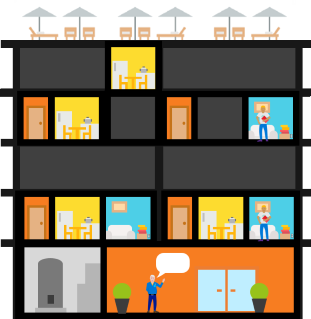
\includegraphics[width=.7\linewidth]{img/apartment_1}
  \\Дом\\(Операционная система)
\end{minipage}
\end{figure}
\end{frame}



\begin{frame}[fragile]
\frametitle{Реализация виртуальной машины и контейнера}
\begin{center}  
	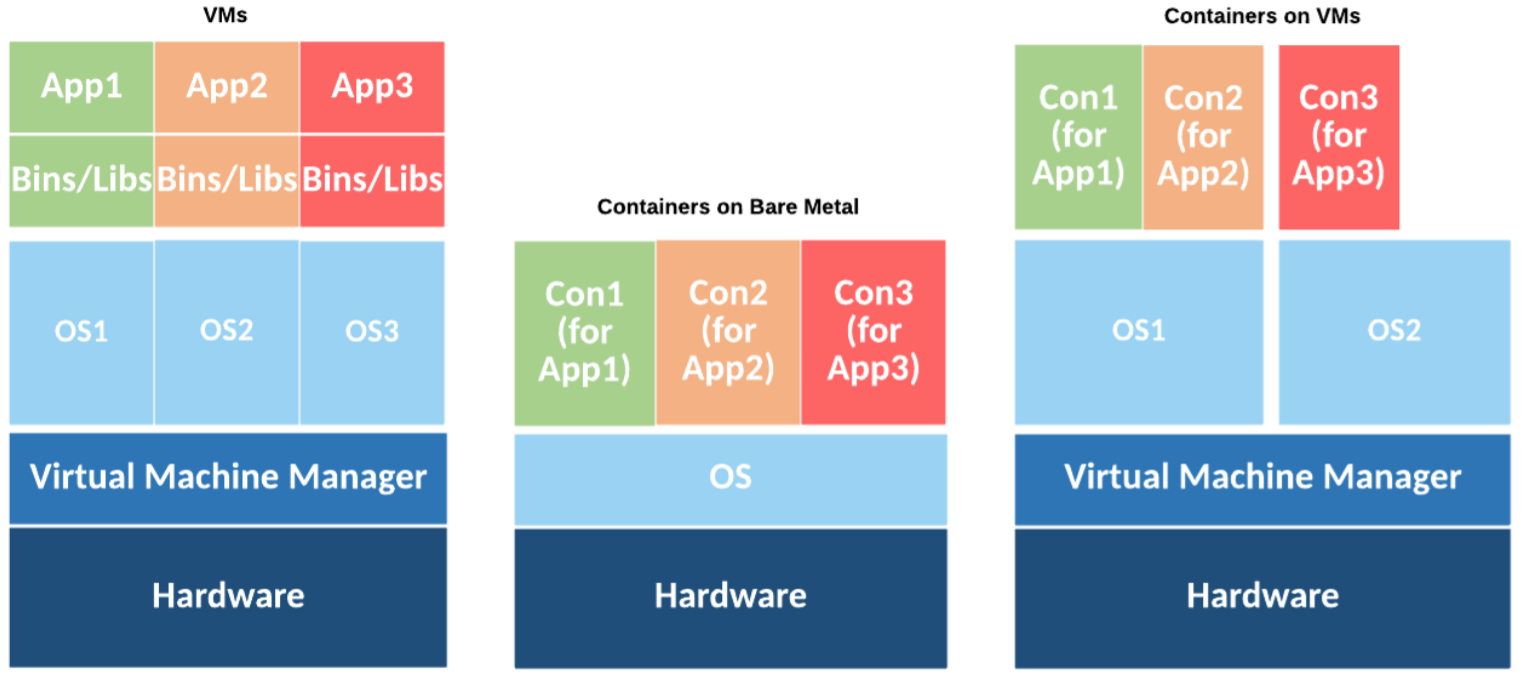
\includegraphics[width=\textwidth]{img/1}
	Сравнение реализаций виртуальной машины и контейнера
\end{center}
\end{frame}



\begin{frame}[fragile]
\frametitle{Типы контейнеров}
LPAC является частным случаем Application Container.
\begin{itemize}
\item \textbf{AC} - Application Container
\begin{itemize}
\item Появился в Windows Server 2016;
\item Разработчики были вдохновлены успехами Docker(Linux).
\end{itemize}
\item \textbf{LPAC} - Less Privileged Application Container
\begin{itemize}
\item Появился в Windows 10 Creators Update(2017 год).
\end{itemize}
\end{itemize}

\end{frame}


\begin{frame}[fragile]
\frametitle{Изоляция LPAC}
Когда приложение запущено внутри LPAC, все разрешения ему требуется выдавать явно. 

На процесс накладываются следующие ограничения доступа:
\begin{itemize}
\item К устройствам(микрофон, камера, принтер...);
\item Файлам системы(чтение, запись);
\item Процессам(межпроцессные взаимодействия);
\item Сети(использование сетевых интерфейсов).
\end{itemize}
\end{frame}


\section{ПРАКТИКА}
\begin{frame}[fragile]
\frametitle{Порядок запуска}
Для запуска LPAC контейнера необходимо:
\begin{enumerate}
\item Создать контейнер, с помощью функции \textbf{CreateAppContainerProfile};
\item $[$Опционально$]$ Установка общих доступов, с помощью функции \textbf{CreateWellKnownSid};
\item $[$Опционально$]$ Установка конкретных доступов, например для файлов используя функцию \textbf{SetEntriesInAclA};
\item $[$Опционально$]$ Изменение переменных окружения, с помощью функции \textbf{ExpandEnvironmentStringsA};
\item Запуск программы, с помощью \textbf{CreateProcessA}.
\end{enumerate}
\end{frame}


\begin{frame}[fragile]
\frametitle{Создание контейнера}
\begin{lstlisting}[language={}, caption={Прототип CreateAppContainerProfile}]
HRESULT WINAPI CreateAppContainerProfile(
  _In_  PCWSTR              pszAppContainerName,
  _In_  PCWSTR              pszDisplayName,
  _In_  PCWSTR              pszDescription,
  _In_  PSID_AND_ATTRIBUTES pCapabilities,
  _In_  DWORD               dwCapabilityCount,
  _Out_ PSID                *ppSidAppContainerSid
);
\end{lstlisting}

\begin{lstlisting}[language={}, caption={Прототип DeriveAppContainerSidFromAppContainerName}]
HRESULT WINAPI DeriveAppContainerSidFromAppContainerName(
  _In_  PCWSTR pszAppContainerName,
  _Out_ PSID   *ppsidAppContainerSid
);
\end{lstlisting}
Затем идет вызов \textbf{UpdateProcThreadAttribute}.
\end{frame}


\begin{frame}[fragile]
\frametitle{Security Identifier (SID)}
\textbf{Security Identifier (SID)} — идентификатор безопасности, структура данных в Windows, которая может идентифицировать системные объекты, например элементы управления доступом (Access Control Entries, ACE), токены доступа (Access Token), дескрипторы безопасности (Security Descriptor). SID всегда начинается с буквы S, далее идут числа, которые обозначают номер редакции ОС, источники выдачи, удостоверяющие центры и другую информацию.\\\\
HKEY\_CURRENT\_USER/Software/Classes/Local Settings/Software/Microsoft/Windows/ CurrentVersion/AppContainerStorage/Mappings
\end{frame}

\begin{frame}[fragile]
\frametitle{Установка общих доступов}
\begin{lstlisting}[language={}, caption={Прототип CreateWellKnownSid}]
BOOL WINAPI CreateWellKnownSid(
  _In_      WELL_KNOWN_SID_TYPE WellKnownSidType,
  _In_opt_  PSID                DomainSid,
  _Out_opt_ PSID                pSid,
  _Inout_   DWORD               *cbSid
);
\end{lstlisting}
\textbf{WELL\_KNOWN\_SID\_TYPE} - идентификатор безопасности (имеется 94 идентификатора).
\begin{lstlisting}[language={}, caption={Структура SECURITY\_CAPABILITIES}]
typedef struct _SECURITY_CAPABILITIES {
  SID                  AppContainerSid;
  PSID_AND_ATTRIBUTES  Capabilities;
  DWORD                CapabilityCount;
  DWORD                Reserved;
} SECURITY_CAPABILITIES, *PSECURITY_CAPABILITIES;
\end{lstlisting}
\end{frame}

\begin{frame}[fragile]
\frametitle{Установка общих доступов}
\begin{lstlisting}[language={}, caption={Прототип UpdateProcThreadAttribute}]
BOOL WINAPI UpdateProcThreadAttribute(
  _Inout_   LPPROC_THREAD_ATTRIBUTE_LIST lpAttributeList,
  _In_      DWORD                        dwFlags,
  _In_      DWORD_PTR                    Attribute,
  _In_      PVOID                        lpValue,
  _In_      SIZE_T                       cbSize,
  _Out_opt_ PVOID                        lpPreviousValue,
  _In_opt_  PSIZE_T                      lpReturnSize
);
\end{lstlisting}
\begin{itemize}
\item \textbf{Attribute} - PROC\_THREAD\_ATTRIBUTE\_SECURITY\_CAPABILITIES - означает, что следующий, созданный процесс будет создан в контейнере;
\item \textbf{lpValue} - структура SECURITY\_CAPABILITIES.
\end{itemize}

\end{frame}

\begin{frame}[fragile]
\frametitle{Изменение переменных окружения}
\begin{lstlisting}[language={}, caption={Прототип SetEnvironmentVariable}]
BOOL WINAPI SetEnvironmentVariable(
  _In_     LPCTSTR lpName,
  _In_opt_ LPCTSTR lpValue
);
\end{lstlisting}
\begin{lstlisting}[language={}, caption={Прототип ExpandEnvironmentStrings}]
DWORD WINAPI ExpandEnvironmentStrings(
  _In_      LPCTSTR lpSrc,
  _Out_opt_ LPTSTR  lpDst,
  _In_      DWORD   nSize
);
\end{lstlisting}
\begin{itemize}
\item \textbf{SetEnvironmentVariable} - установка/перезапись переменной;
\item \textbf{ExpandEnvironmentStrings} - получение значения переменной.
\end{itemize}
\end{frame}

\begin{frame}[fragile]
\frametitle{Установка конкретных доступов к файлам}
\begin{lstlisting}[language={}, caption={Структура EXPLICIT\_ACCESS}]
typedef struct _EXPLICIT_ACCESS {
  DWORD       grfAccessPermissions;
  ACCESS_MODE grfAccessMode;
  DWORD       grfInheritance;
  TRUSTEE     Trustee;
} EXPLICIT_ACCESS, *PEXPLICIT_ACCESS;
\end{lstlisting}
\begin{lstlisting}[language={}, caption={Структура TRUSTEE }]
typedef struct _TRUSTEE {
  PTRUSTEE                   pMultipleTrustee;
  MULTIPLE_TRUSTEE_OPERATION MultipleTrusteeOperation;
  TRUSTEE_FORM               TrusteeForm;
  TRUSTEE_TYPE               TrusteeType;
  LPCH                       ptstrName;
} TRUSTEE, *PTRUSTEE;
\end{lstlisting}
\end{frame}


\begin{frame}[fragile]
\frametitle{Установка конкретных доступов к файлам}
Получение дескриптора безопасности
\begin{lstlisting}[language={}, caption={Прототип GetNamedSecurityInfo}]
DWORD WINAPI GetNamedSecurityInfo(
  _In_      LPTSTR               pObjectName,
  _In_      SE_OBJECT_TYPE       ObjectType,
  _In_      SECURITY_INFORMATION SecurityInfo,
  _Out_opt_ PSID                 *ppsidOwner,
  _Out_opt_ PSID                 *ppsidGroup,
  _Out_opt_ PACL                 *ppDacl,
  _Out_opt_ PACL                 *ppSacl,
  _Out_opt_ PSECURITY_DESCRIPTOR *ppSecurityDescriptor
);
\end{lstlisting}
В возращаемом указателе \textbf{ppDacl} права для объекта.
\end{frame}


\begin{frame}[fragile]
\frametitle{Установка конкретных доступов к файлам}
\begin{lstlisting}[language={}, caption={Структура SetEntriesInAcl}]
DWORD WINAPI SetEntriesInAcl(
  _In_     ULONG            cCountOfExplicitEntries,
  _In_opt_ PEXPLICIT_ACCESS pListOfExplicitEntries,
  _In_opt_ PACL             OldAcl,
  _Out_    PACL             *NewAcl
);
\end{lstlisting}
\end{frame}


\begin{frame}[fragile]
\frametitle{Установка конкретных доступов к файлам}
Установка обновленного дескриптора через \textbf{pDacl}.
\begin{lstlisting}[language={}, caption={Структура SetNamedSecurityInfo}]
DWORD WINAPI SetNamedSecurityInfo(
  _In_     LPTSTR               pObjectName,
  _In_     SE_OBJECT_TYPE       ObjectType,
  _In_     SECURITY_INFORMATION SecurityInfo,
  _In_opt_ PSID                 psidOwner,
  _In_opt_ PSID                 psidGroup,
  _In_opt_ PACL                 pDacl,
  _In_opt_ PACL                 pSacl
);
\end{lstlisting}
\end{frame}



\begin{frame}[fragile]
\frametitle{Запуск программы}

\begin{lstlisting}[language={}, caption={Прототип CreateProcessA}]
BOOL WINAPI CreateProcess(
  _In_opt_    LPCTSTR               lpApplicationName,
  _Inout_opt_ LPTSTR                lpCommandLine,
  _In_opt_    LPSECURITY_ATTRIBUTES lpProcessAttributes,
  _In_opt_    LPSECURITY_ATTRIBUTES lpThreadAttributes,
  _In_        BOOL                  bInheritHandles,
  _In_        DWORD                 dwCreationFlags,
  _In_opt_    LPVOID                lpEnvironment,
  _In_opt_    LPCTSTR               lpCurrentDirectory,
  _In_        LPSTARTUPINFO         lpStartupInfo,
  _Out_       LPPROCESS_INFORMATION lpProcessInformation
);
\end{lstlisting}
\end{frame}




\section{ЭКСПЕРИМЕНТЫ}

\begin{frame}[fragile]
\frametitle{Способ тестирования}
\begin{lstlisting}[language={}, caption={Фрагмент кода, по проверки работы в контейнере}]
OpenProcessToken(GetCurrentProcess(), TOKEN_QUERY, &process_token);

if (!GetTokenInformation(process_token, TokenIsAppContainer, &is_container, sizeof(is_container), &return_length))
    return false;
return true;
\end{lstlisting}
Если приложение в песочнице, провести эксперименты с:
\begin{itemize}
\item переменными окружения;
\item файлами;
\item сетью;
\item проверкой изоляции.
\end{itemize}
\end{frame}

\begin{frame}[fragile]
\frametitle{Изменение переменных окружения}
\begin{lstlisting}[language={}, caption={Фрагмент кода, по изменению переменных окружения}]
SetEnvironmentVariable(L"testName", L"testValue");
	
SetEnvironmentVariable(L"USERDOMAIN", L"HELLOWORLD");

ExpandEnvironmentStringsA("%temp%", path, MAX_PATH - 1);
printf("New path of %%temp%%: %s\n", path);

ExpandEnvironmentStringsA("%localappdata%", path, MAX_PATH - 1);
printf("New path of %%localappdata%%: %s\n", path);
\end{lstlisting}
\end{frame}

\begin{frame}[fragile]
\frametitle{Process Explorer}
\begin{center}  
	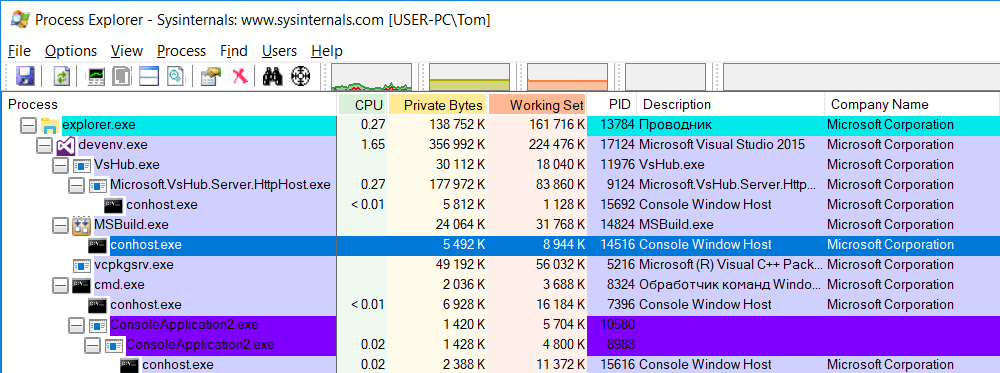
\includegraphics[width=\textwidth]{img/2}
	Древовидная стрктура процессов
\end{center}
\end{frame}

\begin{frame}
\frametitle{Сравнение переменных окружения}
\vspace*{8em}
\begin{center}
\fullsizegraphic{img/3}
\end{center}
\end{frame}


\begin{frame}[fragile]
\frametitle{Доступ к файлам}
\begin{lstlisting}[language={}, caption={Фрагмент кода, по доступу к файлам}]
EXPLICIT_ACCESS_A explicit_access;
explicit_access.grfAccessMode = GRANT_ACCESS;
explicit_access.grfAccessPermissions = FILE_ALL_ACCESS;
...
GetNamedSecurityInfoA(object_name, object_type, DACL_SECURITY_INFORMATION, NULL, NULL, &original_acl, NULL, NULL);
SetEntriesInAclA(1, &explicit_access, original_acl, &new_acl);
SetNamedSecurityInfoA(object_name, object_type, DACL_SECURITY_INFORMATION, NULL, NULL, new_acl, NULL);
\end{lstlisting}
\begin{lstlisting}[language={}, caption={Результат}]
Opening of file C:\Users\Tom\AppData\Local\Packages\mysandboxtest\AC\Temp\allowed_test.txt was successful
Opening of file C:\Users\Tom\desktop\allowed_test.txt was successful
Opening of file C:\Users\Tom\desktop\blocked_test.txt returned access denied
\end{lstlisting}
\end{frame}


\begin{frame}[fragile]
\frametitle{Проверка доступ к сети}
Тестирование будет производиться путем открытия 80 порта, к следующим адреса:
\begin{itemize}
\item \textbf{108.177.14.138} (google.com);
\item \textbf{192.168.1.1} (локальный адрес роутера).
\end{itemize}
Тесты будут выполнены с использованием следующих: WELL\_KNOWN\_SID\_TYPE:
\begin{itemize}
\item WinCapabilityPrivateNetworkClientServerSid - доступ к локальной сети;
\item WinCapabilityInternetClientServerSid - доступ к сети "Интернет".
\end{itemize}
\end{frame}


\begin{frame}[fragile]
\frametitle{Проверка доступ к сети}
Без задачи каких-либо WELL\_KNOWN\_SID\_TYPE:
\begin{lstlisting}[language={}, caption={Полный запрет сети}]
Connection to 108.177.14.138 was blocked
Connection to 192.168.1.1 was blocked
\end{lstlisting}
WinCapabilityPrivateNetworkClientServerSid:
\begin{lstlisting}[language={}, caption={Доступ только к локальной сети}]
Connection to 108.177.14.138 was blocked
Connection to 192.168.1.1 was successful
\end{lstlisting}
\end{frame}


\begin{frame}[fragile]
\frametitle{Проверка доступ к сети}
WinCapabilityInternetClientServerSid:
\begin{lstlisting}[language={}, caption={Доступ только к сети "Интернет"}]
Connection to 108.177.14.138 was successful
Connection to 192.168.1.1 was blocked
\end{lstlisting}
Вместе:
\begin{lstlisting}[language={}, caption={Полный доступ к сети}]
Connection to 108.177.14.138 was successful
Connection to 192.168.1.1 was successful
\end{lstlisting}
\end{frame}


\begin{frame}[fragile]
\frametitle{Список процессов}
\begin{lstlisting}[language={}, caption={Список процессов из изолированного процесса}]
Found process: [System Process]
Found process: ConsoleApplication2.exe
Found process: conhost.exe
\end{lstlisting}
\begin{lstlisting}[language={}, caption={Список процессов из обычного процесса}]
Found process: [System Process]
Found process: System
Found process: smss.exe
Found process: csrss.exe
Found process: wininit.exe
Found process: services.exe
Found process: lsass.exe
Found process: svchost.exe
Found process: WUDFHost.exe
Found process: fontdrvhost.exe
Found process: svchost.exe
Found process: WUDFHost.exe
Found process: svchost.exe
...
\end{lstlisting}
\end{frame}


\begin{frame}[fragile]
\frametitle{Запуск прочих программ}
\tabulinesep = 1mm
\begin{longtabu} to \textwidth {|X[ c , m ] |X[2, c , m ] |}\firsthline\hline
\textbf{Название}&\textbf{Работоспособность}\\ \hline \endfirsthead
Консоль&\cellcolor{green} \\ \hline
Блокнот&\cellcolor{green} \\ \hline
UltraISO&\cellcolor{yellow}\\ \hline
Process Explorer&\cellcolor{yellow}\\ \hline
Internet Explorer&\cellcolor{red}\\ \hline
Google Chrome&\cellcolor{red}\\ \hline
\end{longtabu}
\end{frame}


\begin{frame}[fragile]
\frametitle{Запуск Process Explorer}
\begin{center}  
	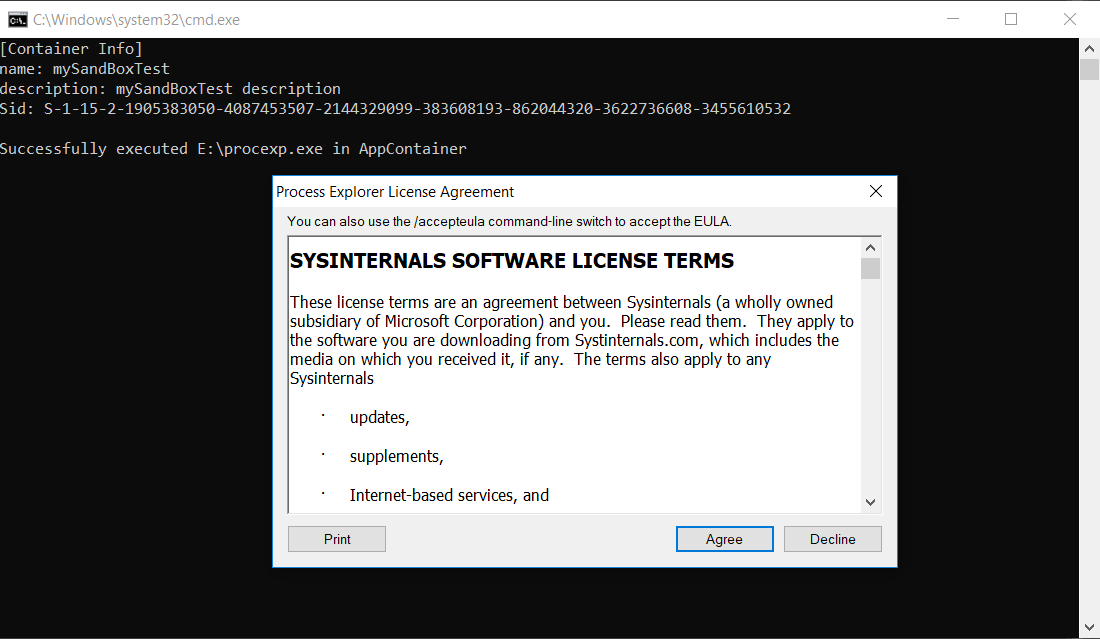
\includegraphics[width=\textwidth]{img/4}
\end{center}
\end{frame}

\begin{frame}[fragile]
\frametitle{Запуск Process Explorer}
\begin{center}  
	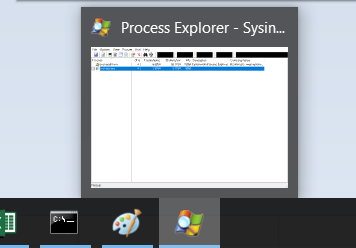
\includegraphics[width=.8\textwidth]{img/5}
\end{center}
\end{frame}


\begin{frame}[fragile]
\frametitle{Реакция системы}
\begin{center}  
	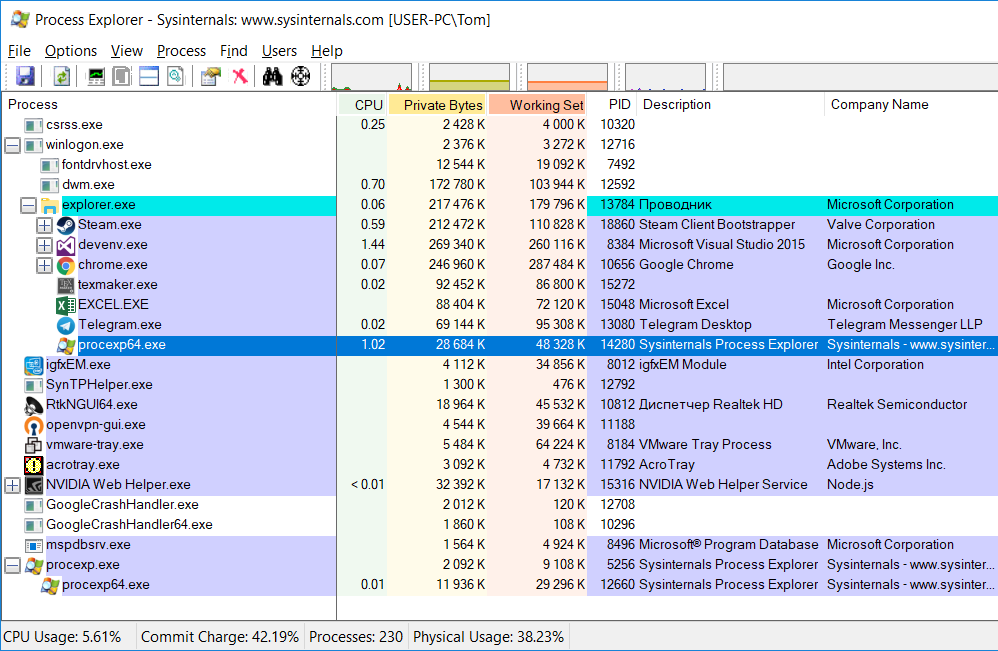
\includegraphics[width=\textwidth]{img/6}
	Состояние после закрытия родительского процесса
\end{center}
\end{frame}

\begin{frame}[fragile]
\frametitle{Работа UltraISO}
\begin{center}  
	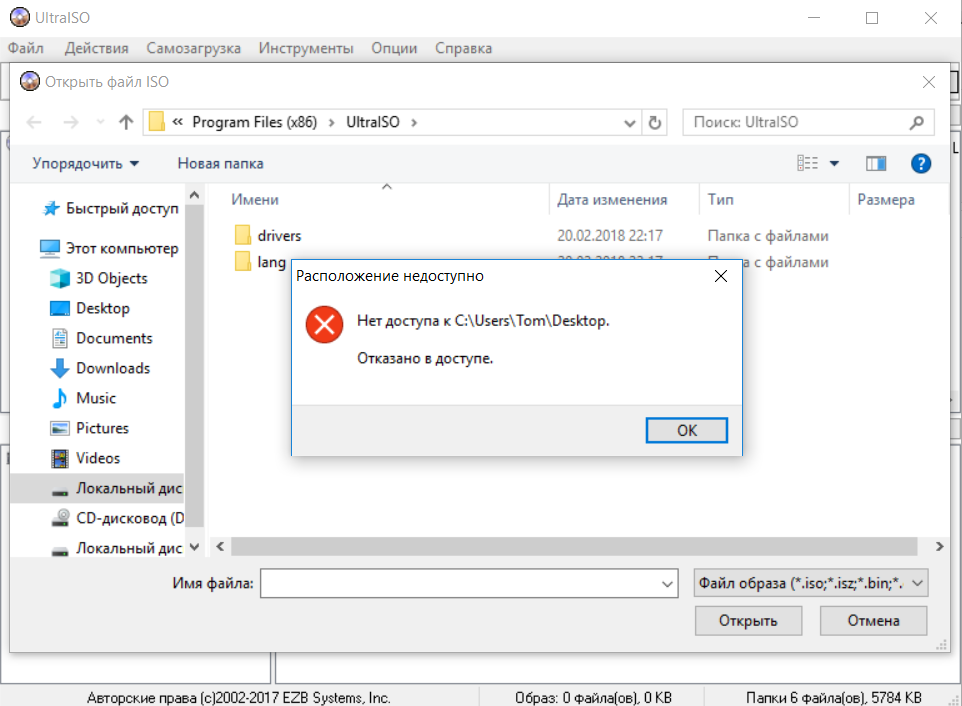
\includegraphics[width=.9\textwidth]{img/7}
\end{center}
\end{frame}


\begin{frame}[fragile]
\frametitle{Работа UltraISO}
\begin{center}  
	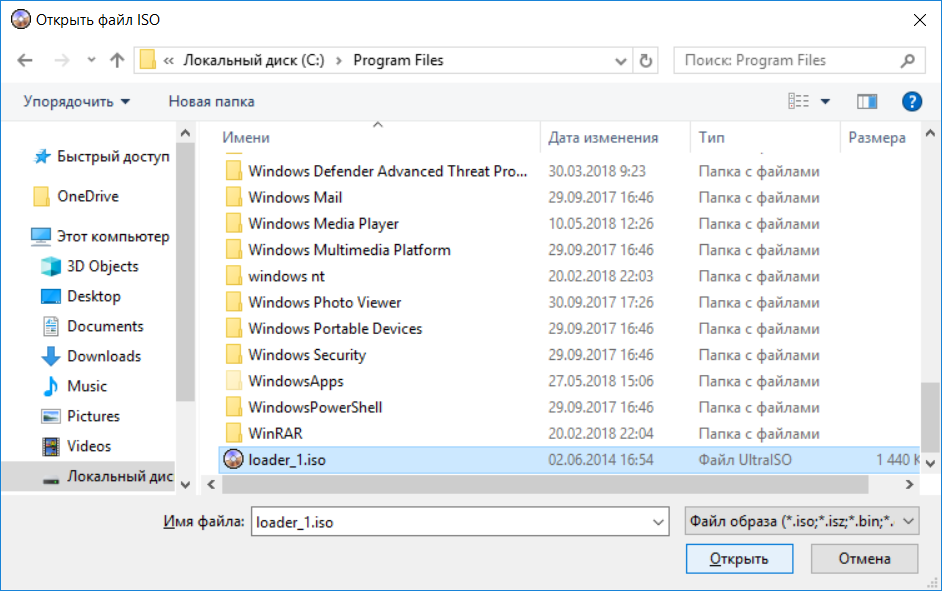
\includegraphics[width=\textwidth]{img/11}
\end{center}
\end{frame}

\begin{frame}[fragile]
\frametitle{Работа UltraISO}
\begin{center}  
	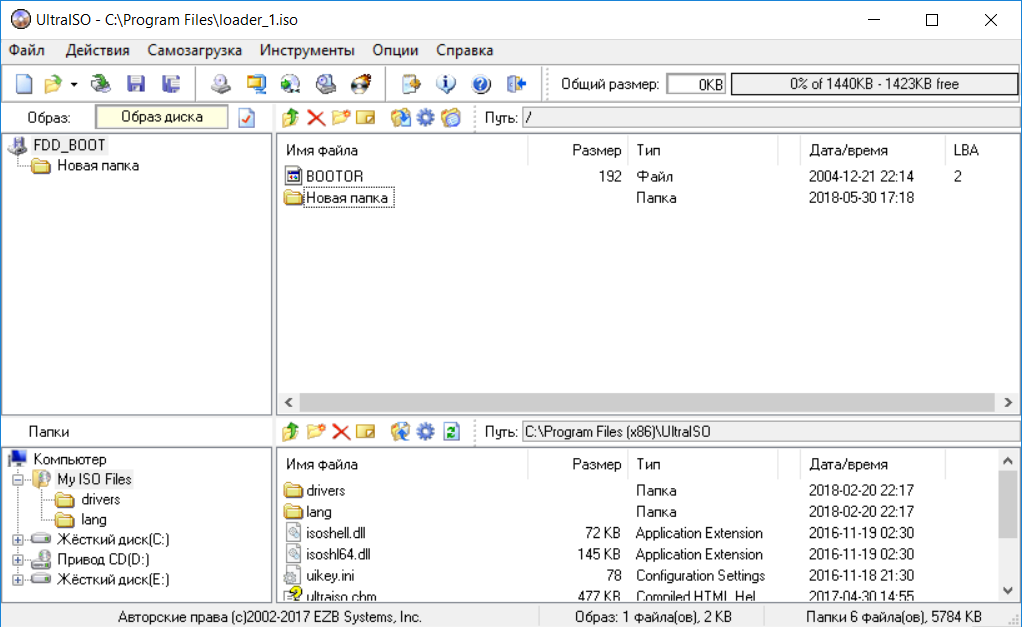
\includegraphics[width=\textwidth]{img/12}
\end{center}
\end{frame}

\begin{frame}[fragile]
\frametitle{Работа UltraISO}
\begin{center}  
	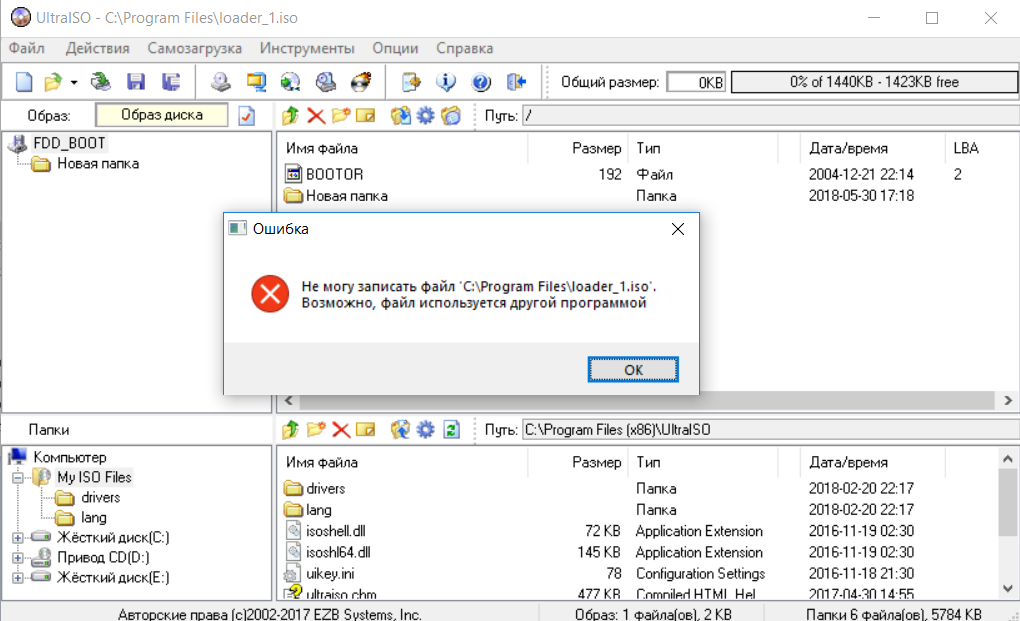
\includegraphics[width=\textwidth]{img/13}
\end{center}
\end{frame}

\begin{frame}[fragile]
\frametitle{Работа UltraISO}
\begin{center}  
	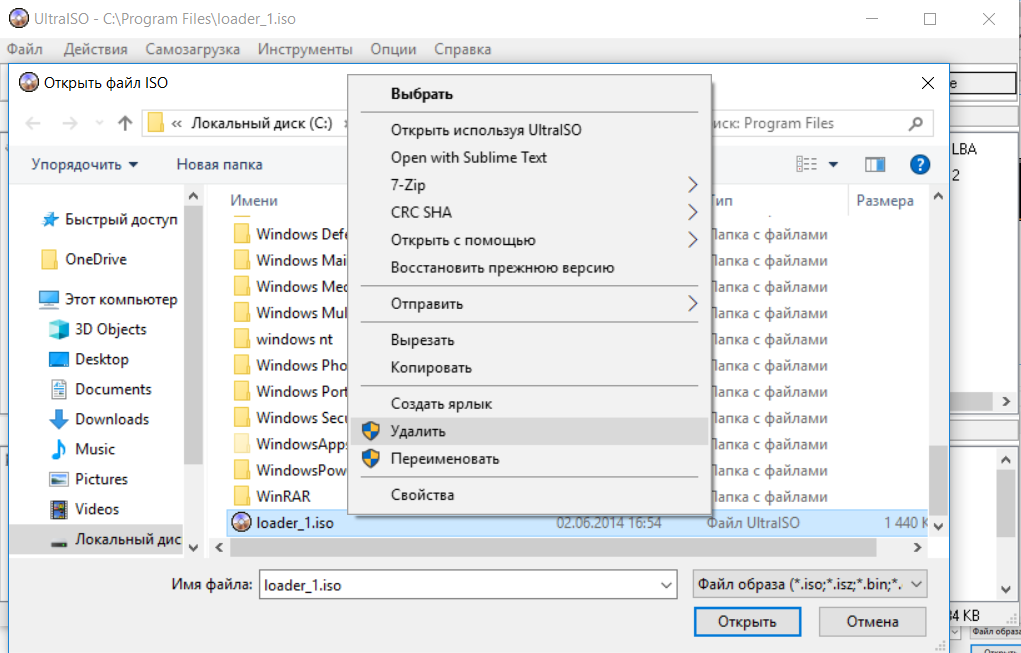
\includegraphics[width=\textwidth]{img/14}
\end{center}
\end{frame}

\begin{frame}[fragile]
\frametitle{Работа UltraISO}
\begin{center}  
	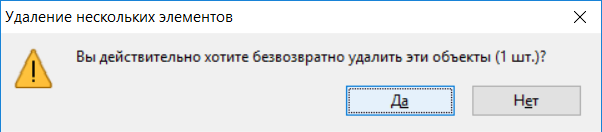
\includegraphics[width=\textwidth]{img/15}
\end{center}
\end{frame}


\begin{frame}[fragile]
\frametitle{Работа UltraISO}
\begin{center}  
	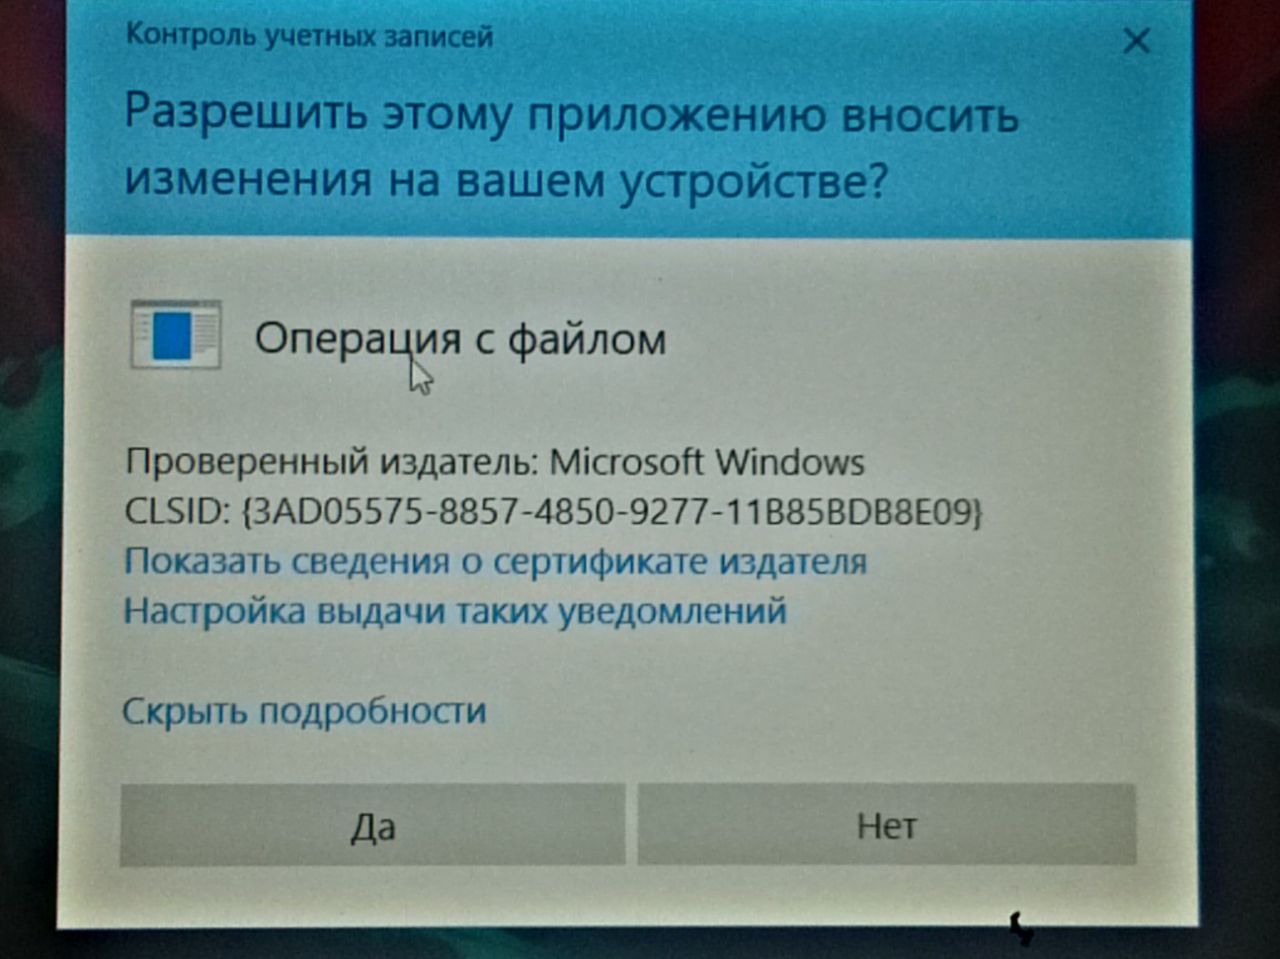
\includegraphics[width=.9\textwidth]{img/16}
\end{center}
\end{frame}

\begin{frame}[fragile]
\frametitle{Работа UltraISO}
\begin{center}  
	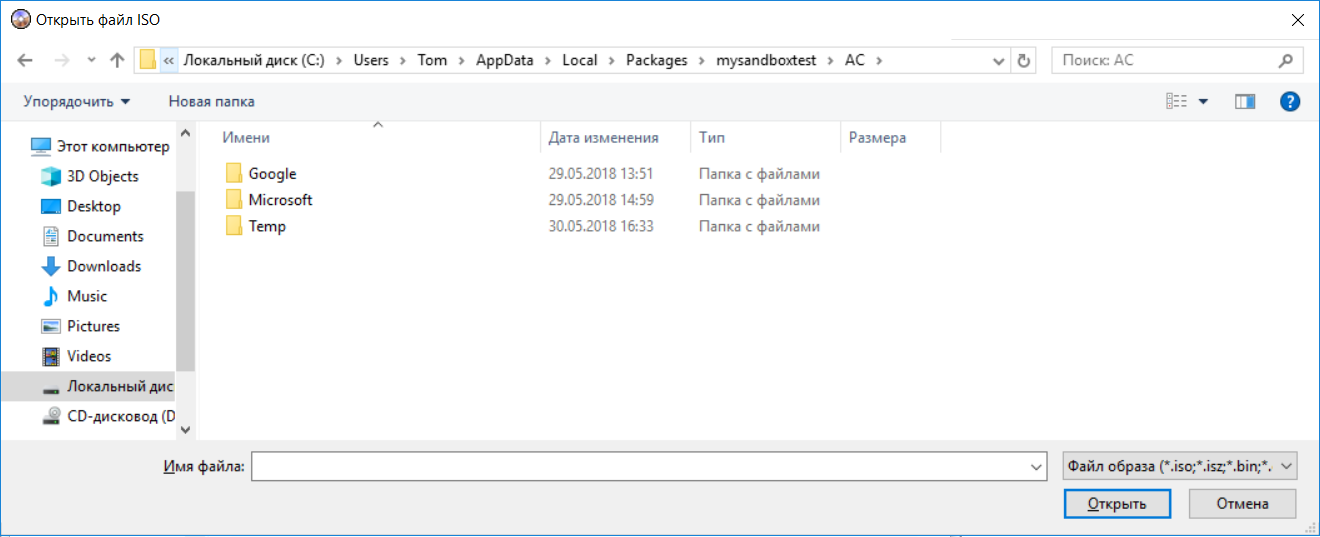
\includegraphics[width=\textwidth]{img/9}
\end{center}
\end{frame}

\begin{frame}[fragile]
\frametitle{Сравнение свойств файлов}
\begin{center}  
	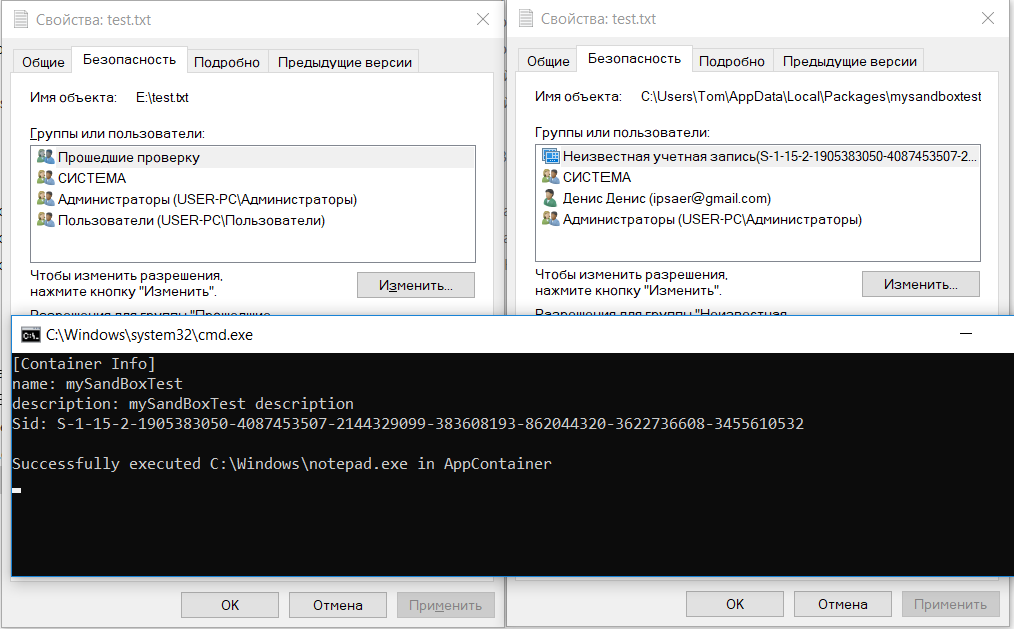
\includegraphics[width=\textwidth]{img/10}
\end{center}
\end{frame}

\begin{frame}[fragile]
\frametitle{Трудности применения LPAC}
\begin{itemize}
\item проблемы с GUI(работает несколько иначе);
\item запуск любого не примитивного приложения является отдельной, достаточно трудоемкой задачей
\begin{itemize}
\item зависимость от прочих сервисов;
\item зависимость от настроек реестра и прочих файлов (то что происходит во время установки)
\end{itemize}
\item трудность выявления ошибок, многие приложения вовсе не сигнализируют об ошибках;
\item LPAC является сравнительно новым инструментом, и слабо документирован.
\end{itemize}
\end{frame}

\begin{frame}[fragile]
\frametitle{Потребитель}
\begin{center}  
	
\includegraphics[width=\textwidth]{img/17}
\end{center}
\end{frame}


\begin{frame}[fragile]
\frametitle{Список использованных источников}
\begin{itemize}
\item https://msdn.microsoft.com/en-us/library/windows/desktop/hh448541(v=vs.85).aspx
\item https://msdn.microsoft.com/ru-ru/library/windows/desktop/aa446585(v=vs.85).aspx
\item https://msdn.microsoft.com/en-us/library/windows/desktop/ms686880(v=vs.85).aspx
\item https://msdn.microsoft.com/ru-ru/library/windows/desktop/ms724265(v=vs.85).aspx
\item https://msdn.microsoft.com/ru-ru/library/windows/desktop/aa446645(v=vs.85).aspx
\item https://msdn.microsoft.com/ru-ru/library/windows/desktop/aa379576(v=vs.85).aspx
\item https://msdn.microsoft.com/ru-ru/library/windows/desktop/ms686206(v=vs.85).aspx
\end{itemize}
\end{frame}

\begin{frame}[fragile]
\frametitle{Список использованных источников}
\begin{itemize}
\item https://msdn.microsoft.com/ru-ru/library/windows/desktop/ms724265(v=vs.85).aspx
\item https://docs.microsoft.com/ru-ru/virtualization/windowscontainers/about/
\item https://nvlpubs.nist.gov/nistpubs/specialpublications/nist.sp.800-190.pdf
\end{itemize}
\end{frame}




\end{document}
